\chapter{Implementation Details}
\label{chap:implementation}
This chapter explains several technical implementation details. It starts with explanation of the bytecode parsing and instrumentation at the native agent part of the complete tool. The following section covers relevant parts of the instrumentation server which are the instrumentation together with creation of transformers and estimators. This chapter ends with a brief explanation of how the spans are exported to the Zipkin user interface and also, how the spans can be exported to a custom data format.
\section{Span and Trace Trees}
This section explains two implementation specific areas related to spans and trace trees. It describes span exporters in more detail and later gives  an overview of the Trace Context API. 
\subsection{Span Exporters}
\label{imp:exporter}
Implementation of span exporters have to extend from the abstract ancestor defining common methods for each span exporter. Also, in order to be able to use the exporter automatically in the code, it has to have a constructor with single \texttt{String} argument accepting exporter arguments. The arguments format is defined in the case of default span exporters, however the developer may use any format in case of custom span exporters. \texttt{SpanExporter} abstract class is the common ancestor for each exporter and has two abstract methods:
\begin{itemize}
	\item \texttt{export}. This method is used for exporting the span. Custom span exporters implementation may save the data on local disk or send over network. The destination is not limited by the code. Internally, the \texttt{export} method is called asynchronously in a separated thread to allow asynchronous span exporting, which can lead to a performance benefit.
	\item \texttt{parseAndSetArgs}. The native agent has configuration property, which the user can use to configure arguments for the span exporter. Each span exporter is responsible for parsing its own arguments.
\end{itemize}

As mentioned in the Section \ref{design:exporter}, the Distrace tool provides two default implementations of span exporters:
\begin{itemize}
	\item  \texttt{DirectZipkinExporter} -  This span exporter sends the collected span asynchronously to the user interface right away without storing the data on disk to be collected by any data collection agent. In this case, the functionality of the span exporter and the data collector are handled by this single exporter.
	This span exporter should be used only for demonstration purposes, since it could overload the user interface or network when processing high number of spans, because the Zipkin user interface is not prepared to handle and store large amount of data in the memory. However, this is a default span exporter at this moment.
	
	This exporter accepts a single argument, which is the IP address and port of the Zipkin user interface. The Figure \ref{fig:zipkin_span_exporter} shows, how the Zipkin span exporter is used.
	
	\begin{figure}
		\centering
		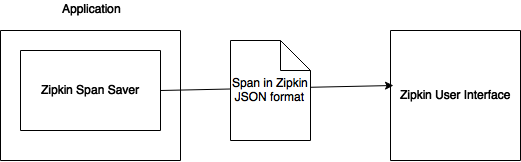
\includegraphics[scale=0.6]{zipkin_span_exporter.png}
		\caption{Using the Zipkin span exporter to export spans directly to Zipkin user interface without the data collection agent.}
		\label{fig:zipkin_span_exporter}
	\end{figure}
	\item  \texttt{JSONDiskExporter} - The second available span exporter saves the collected spans asynchronously on disk in the format known to the Zipkin user interface. The exported spans may be collected in the future by a custom data collection agent and for example, sent to the user interface or database. Together with some well-known data collection agent, this is a preferred way of transferring spans from the application to the Zipkin user interface in the production. This exporter accepts single argument, which is a destination directory for exported spans. The Figure \ref{fig:disk_span_exporter} shows how JSON disk span exporter is used.
	\begin{figure}
		\centering
		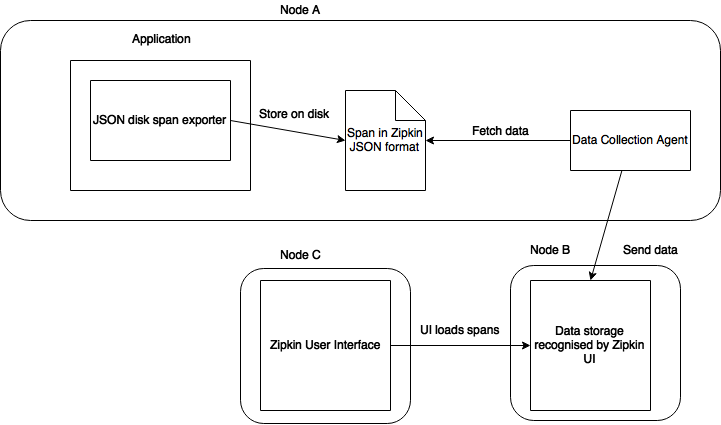
\includegraphics[scale=0.5]{disk_span_exporter.png}
		\caption{Using the JSON disk exporter together with the data collection agent together with the Zipkin user interface .}
		\label{fig:disk_span_exporter}
	\end{figure}
\end{itemize}
Additionally, the Figure \ref{fig:custom_span_exporter} shows how a custom span exporter may be used.

\begin{figure}
	\centering
	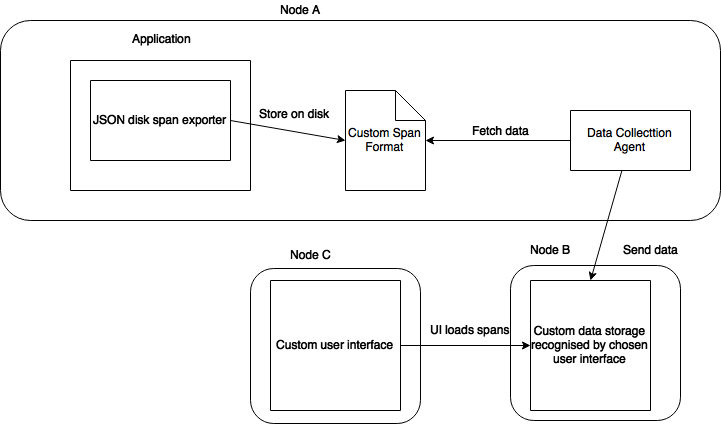
\includegraphics[scale=0.5]{custom_span_exporter.png}
	\caption{Using custom span exporter together with the data collection agent and custom user interface.}
	\label{fig:custom_span_exporter}
\end{figure}

In order to give the developer the flexibility to add new exporters without changing the internals, the custom service loader is used and the span exporters have to be registered in the META-INF directory of the extended instrumentation server JAR file. This ensures that the service loader can find all implementations of the \texttt{SpanExporter} abstract class. The reason why the classes need to be discoverable by the service loader is explained in the Section \ref{desing:native_initialization}.

To make the developer life easier, the \textbf{AutoService} library\footnote{The AutoService library is available at \url{https://github.com/google}.} may used when extending the core server library. Instead of manually registering implementations of custom span exporters into META-INF directory, they can be annotated in the code using the \texttt{AutoService} annotation. This annotation takes a single argument specifying the abstract parent, in this case \texttt{SpanExporter}. The library takes care of registering the classes automatically in the desired folder in correct format so the human error is minimized.

\subsection{Trace Context API}
\label{imp:trace_context_api}
The following methods can be used for obtaining and attaching the trace context:
\begin{itemize}
	\item \texttt{static create()} - creates a new trace context.
	\item \texttt{static getFromObject(holder)} - gets the existing trace context from the holder object.
	\item \texttt{static getFromThread(thread)} - gets the existing trace context from the specified thread.
	\item \texttt{static getFromCurrentThread()} -  gets the existing trace context from the current thread.
	\item \texttt{attachOnObject(holder)} - attaches the trace context to the holder object.
	\item \texttt{attachOnThread(thread)} - attaches the trace context to the specified \newline thread.
	\item \texttt{attachOnCurrentThread()} - attaches the trace context to the current \newline thread.
	\item \texttt{deepCopy} - creates a deep copy of the trace context. It is usually used in cases where child spans are processes in parallel by multiple threads. In this case, the copy of trace context with the same id is shared among all these threads, but they operate on very own objects. This is done in order to allow monitoring of parallel spans within a single trace without having to face race conditions on a single trace context object.
\end{itemize}

The methods above can also be chained and, for example, a trace context can be obtained from the holder object, deep copy created and the newly created copy attached to a new holder object.


\section{Native Agent}
This section covers specific parts of the native agent in more detail. It starts with explanation of considered approaches for instrumentation during the development. The problem of instrumentation server requiring the dependencies for each instrumented class is explained together with the problem of instrumenting the classes with cyclic dependencies. The final solution is explain as well. Further, the instrumentation API, which is used for communication with the server, is explained. Last section describes the byte code parsing.
\subsection{Instrumentation Details}
\label{imp:native:inst}
The native agent does not perform the instrumentation, but asks the server to carry out the transformation. The agent obtains the original bytecode for the class, sends the bytecode to the instrumentation server, waits for the transformed bytecode and lastly, applies the instrumented bytecode.

The instrumentation server requires all dependencies to be available for the the class currently being instrumented. This means that all other classes referenced inside the class file need to be available on the instrumentation server. This includes:
\begin{itemize}
	\item Argument types of all methods.
	\item Return type of all methods.
	\item Type of all fields.
	\item Type of a super class.
	\item Type of implemented interfaces.
\end{itemize}
The dependencies have to be loaded also for the referenced types. To achieve this, we tried two solutions, but only the second solution shown to be feasible.

\subsubsection{Unsuccessful Solution}
The first and unsuccessful solution was based on the fact that several on class file load hooks may be executed at several time in different threads. When the application loads a class, the class load hook event is triggered for it and its bytecode is made available. In this method, the new class file load hook event was artificially enforced via the \texttt{RetransformClasses} method. This method accepts array of classes for which the hook should be re-thrown. In order to continue with the instrumentation of the original class, all dependent classes have to be instrumented in this solution first. This also means that in this approach, the classes with cyclic dependencies are not supported. In order to instrumented such a class, all dependencies have to be instrumented first which is also the class itself.

This solution had also different problem. Since a number of dependencies can be significant, the problem of too many threads being opened at a single time has also appeared. 

\subsubsection{Chosen Solution}
The second and currently used solution is based on the fact that the Java class files may be accessed as a resource using the class loader of the class currently being load. Disadvantage of this solution that the developer may override the \texttt{getResourceAsStream} method on the custom class loader and not provide access to he class files. This is a limitation of the thesis. However, when a such event happens, the instrumentation does not end with the exception but first, the attempt to load the class using a different class loader is done. 

In this solution, the instrumentation server is first asked whether the current class should be instrumented based on the server's extensions. If the class is designed to be instrumented, its bytecode is send to the instrumentation server (only in case if the bytecode for the class is not already available). Then, dependencies are scanned via parsing the raw JVM bytecode which is explained in detail in the following section. Dependency loading is recursively called for each new dependent class until the class does not have any other dependencies or if all the dependencies are already uploaded to the instrumentation server. Once all dependencies for a class have been sent to the server, the instrumentation is invoked and the agent waits for the new bytecode. 

\subsubsection{Auxiliary and Helper Classes}
The instrumentation library used at the server (Byte Buddy) is using so called \texttt{Initializer} class to set up special interceptor field in the instrumented classes. It is a static field which references the instance of the class interceptor - class defining the instrumentation code. This field is automatically set by Byte Buddy framework in most of the cases, but since in case of this thesis the instrumentation is done on different JVM then where the code is actually running, it needs to be handled explicitly. In order to set this field by corresponding \texttt{Initializer} class, both the initializer class and interceptor class need to be available on the agent. The instrumentation server sends the initializer class together with the instance of interceptor during the instrumentation of the class and the agent registers the interceptor and initializers with the instrumented class for later use since the static interceptor field can be set up when the class is used for the first time. The initializers are loaded during  \texttt{Class Prepare} event. This event is triggered when the class is prepared but no code has been execute so for. 


Also several helper classes are sent back to the native agent at the stage where the class is checked whether it should be instrumented or not. The classes are auxiliary Byte Buddy classes and also instances of \texttt{LoadedTypeInitializer} class. The initializers are sent as serialized 
instances and therefore their defining class has to be available in the application. This is achieved in the agent initialization phase where several required classes are sent to the application from the server. The instances are saved to a map which maps the initializer name to its serialized representation. This initializer is later using during the class preparation phase to set the static interceptor field of the instrumented class as mentioned in the previous sections.

The callback for \texttt{Prepare} event is also used to register the native methods for the class being loaded. Registering the native method to the class makes it available from Java programming language.

The auxiliary classes are classes created at run-time during the instrumentation on the server and have to be available on the applications machine as well. This is achieved by loading the bytecode for the auxiliary class, saving the class as a java class file on the disk and making it available by adding the class on the application's class path.

\subsection{Instrumentation API}
The Instrumentation API provides several methods used to communicate with the instrumentation server. It provides low-level methods for sending data in form of byte arrays or strings and the corresponding methods for receiving the data. On top of these method several methods are built to make the communication easier. The most important methods are:
\begin{itemize}
	\item \texttt{sendClassData} method sends bytecode to the instrumentation server.
	\item \texttt{isClassOnInstrumentor} method checks whether the bytecode for the given class is already on the instrumentation server or not.
	\item \texttt{instrument} method triggers the instrumentation and returns the instrumented bytecode.
	\item \texttt{loadInitializersFor} method is for loading the initializers for specific class.
	\item \texttt{loadDependencies} method is used to load all dependent classes and upload them on the instrumentation server. The dependency is uploaded only in case it's not already available on the instrumentation server.
	\item \texttt{shouldContinue} method checks if the class on its input is allowed to be instrumented.
	\item \texttt{loadPrepClasses} method loads all dependent classes in the agent initialization phase.
\end{itemize}

\subsection{Byte Code Parsing}
\label{imp:parsing}
Byte code parsing is necessary feature of the thesis and is required in order to be able to get the list of dependent classes on a class currently being loaded. No sufficient C++ implementation has not been found and therefore a custom parsing module has been implemented. The parsing module is based on the Apache Commons BCEL Java package and the simplified version but still with the same logic has been rewritten to C++.

The main class used for parsing is \texttt{ClassParser} which contains \texttt{parse} method accepting the bytecode of a class and defines also several accessors  for the parsed data such as the super class name and complete reference, list of all implemented interfaces, list of all methods or list of all defined fields and their types.

The bytecode starts with the several important parts:
\begin{itemize}
	\item \textbf{Magic id}. Magic id is a first integer stored in each bytecode and contains  always 0xCAFEBABE number.
	\item \textbf{Version}. This part contains actually two shorts, where the first short represents minor Java version and the later one represents major Java version.
	\item \textbf{Constant pool}. Constant pool is a table representing class and interface names, field names and also other important constants. It contains mapping from id representing the type to the fully qualified type name.
	\item \textbf{Class Info}. Class information contains the information whether the bytecode represents a class or an interface, denotes class name and also super class name.
	\item \textbf{Interfaces}. This part contains the number of interfaces this class implements followed by id of type short of each interface. The interface can be looked up using the class pool.
	\item \textbf{Fields}. This part of the bytecode contains the number of fields this class defines together with some additional information for each defined field.
	\item \textbf{Methods}. This part contains the number of defined methods in the bytecode together wit additional information per each method such as the number of arguments.
\end{itemize}
More information about class file structure can be found at the official Java documentation\footnote{The documentation of the class loading process is available at \url{https://docs.oracle.com/javase/specs/jvms/se7/html/jvms-4.html}}.
Each part of the class file mentioned above is parsed separately. For accessing the raw bytecode a \texttt{ByteReader} class is used. It contains methods fro reading different types of data from the bytecode array. 

Parsing the magic id and both minor and major versions is straightforward as their are just numbers and can be read using the byte reader class directly. Parsing of the constant pool is more complex. For each entry in the constant pool a constant representing the entry is read. The constant can be of several type such as constant representing the Class symbol, String symbol, Method types of Field types for example. Once the Constant pool is parsed, it can be queried for the specific symbol by its id. Class name and super class name, interfaces, fields and methods are read from the constant pool by using their ids.

\section{Instrumentation Server}
\subsection{Instrumentation}
\label{impl:server:instr}
The code to be instrumented is specified using the \texttt{MainAgentBuilder} and \texttt{BaseAgentBuilder} classes.
The instrumentation server expects the instance of \texttt{MainAgentBuilder} on the input of its \texttt{start} method. This is an abstract class containing single abstract method \texttt{createAgent(BaseAgentBuilder builder, String pathToHelperClasses)}, where the builder is a wrapper around the Byte Buddy \texttt{AgentBuilder} class, which is used to define the class transformers.

The developer needs to implement this method and specify on which classes and on which methods the instrumentation should happen. Since Byte Buddy is used for writing transformers and interceptors, please read more about Byte Buddy in the Section \ref{sec:byte_buddy}. The server provides several helper methods for creating the transformers and interceptors, which are less verbose then the standard Byte Buddy approaches.

Each transformer has to have associated either an interceptor or advice defining the code to be injected to the original code. Each interceptor implementation has to implement \texttt{Interceptor} interface. This is required for the server to be able to discover all interceptors at run-time without the need for changing the internals of the server. Each implementation of the interceptor needs to register itself in the META-INF directory of the generated JAR in the same way as the span exporters mentioned in the previous section. Custom service loader is then used to locate all classes implementing the \texttt{Interceptor} interface. 

The advices may be used without any special annotations since Byte Buddy in-lines the code defined by the advices into the original code and therefore there is no need to transfer the Advice classes to monitored application.

Even though Byte Buddy takes care about the internals of the instrumentation, the \texttt{BaseAgentBuilder} class is internally properly configured so the instrumentation is defined exactly as desired. The class implements four Byte Buddy listeners used for informing us about the instrumentation progress and allow us to react on the process of the instrumentation. The listeners are:
\begin{itemize}
	\item \texttt{onTransformation} listener is called immediately before the class is instrumented.  Implementation of the listener in the thesis also sends the agent all auxiliary classes required by the instrumented class and the initializers used for setting the static interceptor field on the instrumented class.
	\item \texttt{onIgnored} listener is called when the class is not instrumented. The class is not instrumented when the user does not define any transformer for the specified class.
	\item \texttt{onError} listener is called when some exception occurred during the instrumentation.
	\item \texttt{onComplete} listener is called when instrumentation process completed. It is called after both of \texttt{onTransformation} and \texttt{onIgnored} listeners.
\end{itemize}

Byte buddy requires dependencies for the instrumented class to be available. They are needed because the instrumentation framework needs to know signature of all methods in several cases, for example when the method is overridden in the child class. The dependencies are all the classes specified in the class file such as type of the methods return value or arguments, super class or implemented interfaces. 
By default, Byte Buddy tries to find these dependencies using two classes - \texttt{LocationStrategy} and \texttt{PoolStrategy}. The first class is used to tell Byte Buddy where to look for the raw bytecode of dependent classes. The classes are loaded by context class loader by default, but since the classes are received over the network, custom \texttt{InstrumentorClassloader} class loader is used to handle the class loading. It is a simple class loader which keeps the cache of the classes received from the agent and when a request for instrumentation comes, instead of looking into the class files, it loads the data from the cache in the memory.

However, Byte Buddy internal API does not work with raw bytecode for scanning the further dependencies and obtaining the metadata for the classes. It uses classes \texttt{TypeDescription} and \texttt{PoolStrategy} for this purpose. The first class has a constructor accepting the \texttt{Class} class and created instance contains metadata for the class such as the signature of all methods and fields, list of all interfaces or for example list of constructors. The second class is used for caching the type descriptions so they are not created every time the class is accessed. 

So in overall, class lookup is done in the following two steps:
\begin{enumerate}
	\item Check whether type description for the class is available. If yes, load the type description from the cache.
	\item If the type description is not available, load the class using the \linebreak \texttt{InstrumentorClassloader}, create type description for the class and put it in the cache.
\end{enumerate}

\subsection{Optimizations}
The instrumentation server does several optimizations to speed the communication with the native agent. The first optimization is caching of the classes sent to the instrumentation server from the native agent and also caching of the already instrumented classes. This behavior is useful in case we are using the shared instrumentation server. In this case multiple native agents are sharing the same instrumentation server. When a class is received from any agent, it is cached and the rest of the native agents don't need to send the original class again. The instrumentation server also performs the instrumentation only once and caches the instrumented class. When any agent requests to instrument already instrumented class on the server, the server just sends the class immediately from the cache.

The other way how the communication can be optimized can be influenced by the user. The user may compile the extended instrumentation server with the application classes or add these classes on the classpath of the server. When a native agent asks the server for instrumenting some class, the server first check if it can load the original class itself locally and avoid sending the bytecode from the native agent. 
\subsection{Span Injection}
This short section explains how additional fields such as the span information are internally attached to the instrumented classes. The trace information is attached to the instrumented class by adding a new synthetic field with name \texttt{\_\_\_\_traceId}. This trace id represents the current trace and is used in the code to obtain reference to a current trace context and also current span.  A new field is created using the Byte Buddy instrumentation builder using the \texttt{defineField} method.
\subsection{Determine the Current Span Exporter}
This section explains how a span exporter type and also other arguments passed to the native agent are made accessible to the instrumentation server. The span exporter type is defined as part of the native agent and needs to be available at the instrumentation server as well. This is achieved by creating and registering the native method to a class, which is defined as part of the instrumentation server.
In case of span exporters, the abstract class \texttt{SpanExporter} is defined at the instrumentation server and contains native native method named \texttt{getSpanExporterType} for getting the span exporter type. The abstract \linebreak \texttt{SpanExporter} class is sent to the native agent during the initialization phase. When this class is required for the first time, the native method implementation is bound to the method \texttt{getSpanExporterType} defined in the \texttt{SpanExporter} class. Therefore, even the classes defined as part of the instrumentation server can use methods defined on the native agent with really small overhead. Actually, there may be a performance gain, since these methods are written as native methods.

\subsection{JSON Generation}
\label{json_gen}
The data inside spans are internally stored as instances of \texttt{JSONValue} class since in order to support the communication with the default Zipkin user interface they need to be exported as JSON. JSON is a lightweight format for exchanging data where the syntax is based on Javascript object notation.

The JSON handling is based on the minimal-json library\footnote{The library is available at \url{https://github.com/ralfstx/minimal-json}.}, however custom simplified implementation was created which fits the theses requirements. Also the number of dependencies is lowered by this decision. 

This JSON support is designed via several classes:
\begin{enumerate}
	\item \textbf{JSONValue}. The abstract ancestor of all JSON types. This type defines common methods to all implementation.
	\item \textbf{JSONString}. Class representing the string type.
	\item \textbf{JSONNumber}. Class representing the numeric types.
	\item \textbf{JSONLiteral}. Class representing the literals \textbf{null}, \textbf{true} and \textbf{false}.
	\item \textbf{JSONArray}. Class representing the JSON arrays. It has support for adding new elements into the array.
	\item \textbf{JSONObject}. Class representing the JSON objects. It has support for adding a new items in the object.
\end{enumerate}

Each \textbf{JSONValue} can be printed as valid JSON string where the printing is driven by\texttt{JSONStringBuilder} class. This class is also responsible for escaping the characters according to JSON standards. The default printer prints the data without any formatting as one line, however \texttt{JSONPrettyStringBuilder} prints the data in more human-readable format. The second printer is usually used for debugging purposes and the first one for real usage as the size of the data is smaller in this case.


